\documentclass[notumble,combine]{leaflet}
\usepackage[dvipsnames,usenames]{color}
\usepackage{graphicx}
\usepackage{alltt}
\usepackage{url}
\usepackage{ascmac}
\usepackage{comment}
\usepackage{here}
\usepackage{wrapfig}

\makeatletter
% from leaflet.cls
\renewcommand\section{\@startsection{section}{1}{\z@}%
  {-3.5ex \@plus -.75ex}%
  {1ex} %{1.5ex}%
  {\normalfont\large\sectfont\color{NavyBlue}}}
\renewcommand\subsection{\@startsection{subsection}{2}{\z@}%
  {-2.5ex plus -.5ex}%
  {1\p@} %{1ex}%
  {\normalfont\normalsize\sectfont\color{BrickRed}}}
\makeatother

\graphicspath{{figures/}} 

\title{
	\includegraphics[width=\textwidth]{kbug-logo}\\
        \parbox[c]{2cm}{\resizebox{2cm}{!}{\textcolor{red}{\bf{@}}}}
	
\includegraphics[width=\textwidth]{KOF2012}\\
	\vfill
	\parbox[c]{4cm}{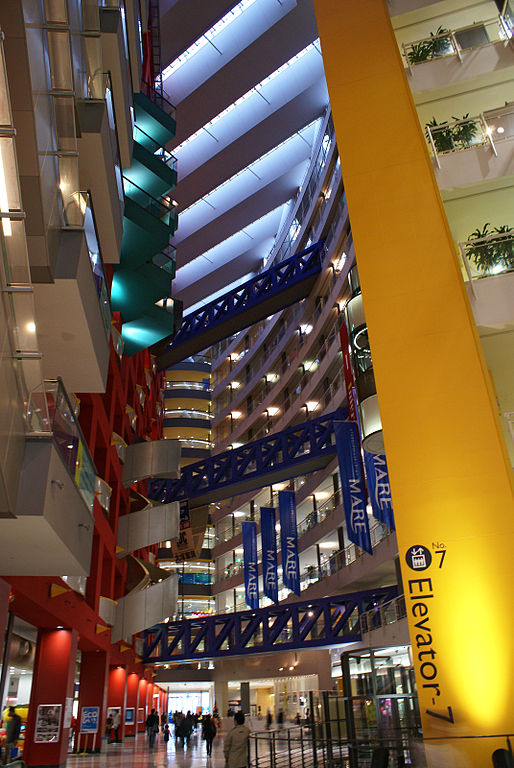
\includegraphics[width=4cm]{514px-Atc_osaka03s3200}}\\
        \hfill{{\footnotesize \copyright 663highland @ Wikipedia-ja}}
        \vfill
	\resizebox{\linewidth}{!}{\bf 関西*BSDユーザ会}\\
        \resizebox{\linewidth}{!}{{\bf \url{http://www.kbug.gr.jp/}}}\\
        \parbox[c]{1cm}{\resizebox{1cm}{!}{\textcolor{Orange}{\bf{@}}}}
        \resizebox{\linewidth}{!}{{\bf \url{http://2012.k-of.jp/}}}\\
        \resizebox{\linewidth}{!}{2012年11月8日(金),9日(土)}\\
}



\date{}

\begin{document}
\maketitle
\thispagestyle{empty}
\pagebreak{}
\section{関西*BSDユーザ会(K*BUG)ってなぁに?}
関西 *BSD ユーザ会 (Kansai *BSD Users Group; K*BUG)とは、
BSD系OSのユーザ同士の情報交換のための{\Large\em \textcolor{red}{場}}で、1999年に設立されました。

年に数度の勉強会やイベントの参加、そして{\Large\em \textcolor{red}{飲み会}}を行っています。

\subsection{K*BSDの基本理念}
K*BUGの基本理念はのとおりです
\footnote{\url{http://www.kbug.gr.jp/charter.html}}。

\fbox{\begin{minipage}{\textwidth}
\begin{itemize}
\item 場の提供を目的とする
\item 人のケツは叩くが足は引っ張らない
\item 来るものは拒まず、猿ものは追わず
\item だれでも役員になれる。誰でも役員は止められる
\end{itemize}
\end{minipage}}

少し難しく感じるかもしれないですが、
\textcolor{red}{BSDへの愛と情熱}
があれば、
あなたが
\textcolor{blue}{やりたいと思うことができる場}
がK*BUGなのです。

\section{K*BUG Keywords}
K*BUGでは、これまで以下のようなKeywordに関する発表や展示を行いました。

{\large\bf\textcolor{red}{{BSD}}} (FreeBSD (PC-BSD), NetBSD, OpenBSD, DragonlyBSD, {\footnotesize Mac OS X(?), iOS(??) }, ...
の更新情報 / 利用方法 / ...,
arch {\footnotesize (i386, amd64, macppc, landisk, zaurus, wzero3, hpcmips, fonera, netwalker, ipaq, fonera, ...)},
kernel hackや新技術 (DTrace, ZFS, シリアルドライバ, ...),
FreeBSD portsってなに?,
Security, 
Prolog, Lisp,
Squeak, Scratch,
OpenCV,
ContaoCMS, 
hardware (UPS, HDD, Server, ...),
ものづくり,
電子工作,
ニコ動技術部 (猫耳サーボ % (USB audio servo controler)
, 鼻ホタル, ...),
雑誌付録基板 ,
Physical Computing (Gainer (gainerm-lib), Arduino, ...),
木彫, でーもんくん, でもんむし君 , \\
{\textcolor{red}{{\bf\large 飲み会}}}, and {\em\textcolor{red}{{ more with }}{\Large\bf\textcolor{red}{{YOU!!}}}}

\section{K*BUGの活動}
最近の活動はこんな感じです。
発表資料URLはここ
\footnote{\url{http://qml.610t.org/FreeBSD/KOF2012.html}}に
あります。
もし、興味のあるテーマがあったら、
\begin{center}
{\huge\bf \textcolor{red}{遊びに来てね!!}}
\end{center}

\subsection{2012年10月20日(土)@大阪 第6回研究会}
\begin{itemize}
\item NetBSD 6.0Rの変更点
\end{itemize}

\subsection{2012年 8月18日(土)@京都 第5回研究会}
\begin{itemize}
\item 新しいレノボPC X230買いました
\item NetBSD on kobo
\item FREQUPS UPF F and NetBSD
\item Multi Thread Tiny BASIC on PIC32 and RetroBSD
\item androidのアプリ
\item Buffaloルータのシリアル
\end{itemize}

\subsection{2012年 8月3日(金), 4日(土) @京都 \\\hfill OSC2012 Kansai@Kyoto}

\begin{itemize}
\item OpenBSDでNAT64
\item RetroBSD展示
\item でーもんくんの行進:
  miniでーもんくん, 
  ダンボールでーもんくん % Arduino
  よろこび棒 OSC2012, ... % OSC2012 Kansai@Kyoto版
\item K*BUG POV (失敗) %with Japanino
\item チラシとでもんむし君シール配布
\end{itemize}

\begin{center}
 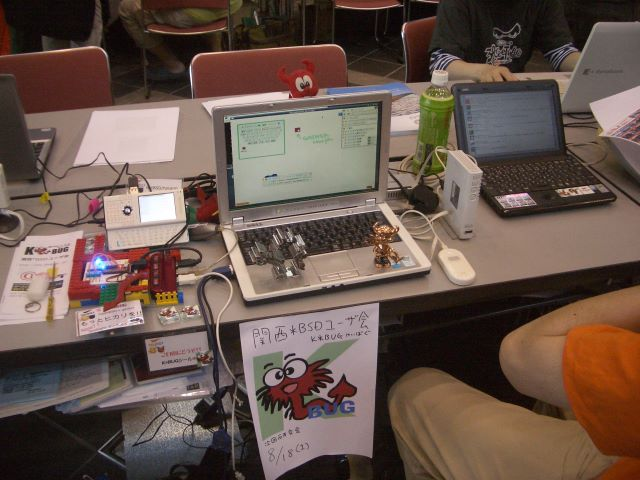
\includegraphics[width=4cm]{osc2012booth}
\end{center}

\subsection{2012年 7月29日(日)イベント@奈良高専\\\hfill 第4回研究会}
K*BUGメンバー参加者、2名だけだったけど、若者が多かったのよろしかったかと。
\begin{itemize}
\item PC-BSDをはじめよう!! %(インストール実習) %\footnote{\url{http://qml.610t.org/FreeBSD/PCBSD.html}}
\item K*BUGをはじめよう!! %\footnote{\url{http://qml.610t.org/FreeBSD/WhatIsKBUG.html}}
\item おしごとBSDを推めよう
\item 展示: RetroBSD, Physical Computing, BSD書籍
\end{itemize}

\begin{center}
 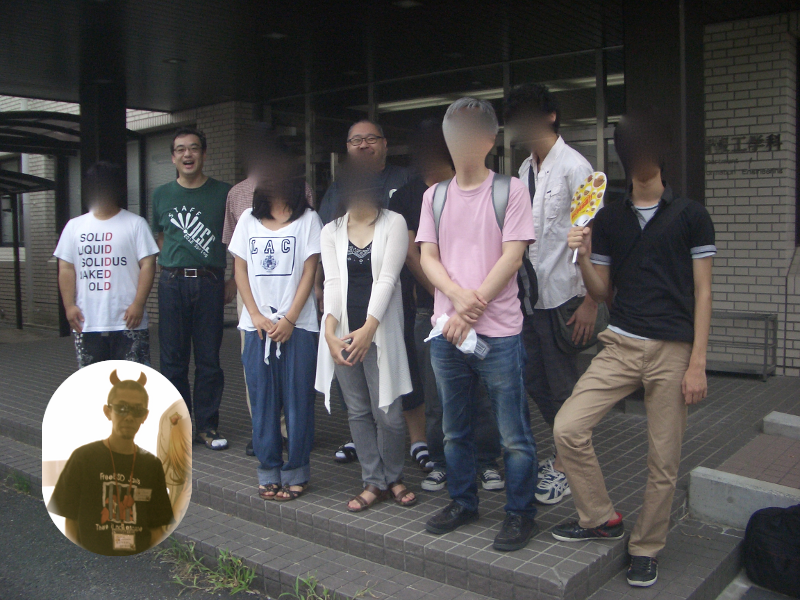
\includegraphics[width=4cm]{event_nnct}
\end{center}

\subsection{2012年 6月23日(土)@大阪 第3回研究会}
\subsection{2012年 4月21日(土)@京都 第2回研究会}
\begin{itemize}
\item Sony NEWSのMOをサルベージする
\item USB memstickで使うFreeBSD
\item n12iさんちのお話
\item FreeBSD portsと暮らす(2) - ports作成編 %\footnote{\url{http://www.slideshare.net/umq_876/making-freebsdports}}
\item FreeBSD portsと暮らす(3) - redportsを使おう %\footnote{\url{http://www.slideshare.net/umq_876/using-redports}}
\item lang/squeak portの更新 %\footnote{\url{http://qml.610t.org/squeak4_4_7_2375.html}}
\item BSDお仕事の会のお話 (BSD-BA) %\footnote{\url{http://www.bsd-ba.org/}}
\end{itemize}
\subsection{2012年 2月18日(土)@大阪 第1回研究会}
\begin{itemize}
\item FreeBSD portsと暮らす(1) - github編 %\footnote{\url{http://www.slideshare.net/umq_876/making-freebsdports}}
\end{itemize}

\subsection{2011年12月17日(土)@大阪 \\\hfill 定期総会+第5回研究会+忘年会}
\begin{itemize}
\item USBガイガーカウンターをつなぐ+USBサウンドI/Fをつくる+USBでデジカメ制御
\item はじめてのNetBSD
\item dnssec authenicated https
\item 2011 K-OF K*BUG出展まとめとこれまでやってみて考えたこと
\end{itemize}

\newpage
\section{BSDに関する情報}
\subsection{BSD開発元リンク}
\begin{itemize}
\item NetBSD情報
  \url{http://www.jp.netbsd.org/}
\item FreeBSD友の会  \url{http://www.jp.freebsd.org/}
\item OpenBSD本家  \url{http://www.openbsd.org/ja/}
\item DragonFly BSD \url{http://dragonflybsd.org/}
\end{itemize}

\subsection{K*BUG関連}
以下のURLなどで、活動が紹介されています。

\begin{minipage}{\textwidth}
\begin{shadebox}
\begin{itemize}
 \item Twitter \url{http://twitter.com/610t/kbug}
 \item いしはら \\\hfill{\small \url{http://www.tunagu.gr.jp/fswiki/isihara/}}
 \item うえだ {\small \url{http://www.ueo.co.jp/~tueda/diary/}}
 \item 西東 \url{http://d.hatena.ne.jp/tunefs/}
 \item 白井 \url{http://hp.vector.co.jp/authors/VA012337/misc/presentation.html}
 \item たけおか \url{http://www.takeoka.org/}
 \item 寺本 \url{http://d.hatena.ne.jp/mteramoto/}
 \item 野田 \url{http://d.hatena.ne.jp/akira_you/}
 \item みつなが \url{http://n.mtng.org/ele/}
 \item むとう \url{http://qml.610t.org/FreeBSD/}
\end{itemize}
\end{shadebox}
\end{minipage}

\section{これからの関連イベント(予定)}
K*BUGでは、だいたい2ヶ月に1度の頻度で勉強会を行っています。
また、主に関西のイベントで、展示などを行っています。

現在、予定されているイベントは、以下のとおりです。
詳細に関しては、K*BUGのWebページをご確認ください。

\begin{itemize} 
\item 2012年12月8日(土)@京都 (AXE会議室) \\ % 学院大学
  第14回定期総会 + 第7回研究会 + 忘年会
\item \textcolor{Gray}{2013年8月(?) OSC2013 Kansai@Kyoto}
\item \textcolor{Gray}{2013年11月(?) KOF2013}
\item \textcolor{Gray}{2013年(?)月 イベント@奈良高専}
\end{itemize}

\newpage
\section{K*BUG @ KOF2012}
BSD使って、以下の様な展示をしています。

\begin{center}
{\huge\bf \textcolor{red}{遊びに来てね!!}}
\end{center}

\begin{itemize}
\item 魅惑の付録基板の世界
\item Physical Computing, 工作でーもんくん
%\item Squeak / Scratch でもI/O
\item でもんむし君シールとチラシ%\footenote{\url{}} 
\textcolor{red}{\Large\em 強制配布!!}
\item JNUG: 我ら絶好調、ちっちゃいものクラブ!!のご相伴
\end{itemize}

\section{BSDなひととき} % by 日本NetBSDユーザーグループ}
\begin{wrapfigure}[8]{r}{2.5cm}
 
\includegraphics[width=2.5cm]{seal2}
\end{wrapfigure}

\begin{itemize}
\item 日時: 2012/11/09(金) 14:00-15:00
\item 会場: 9F セミナールーム2
\item 講師: 蛯原 純 (The NetBSD Project/株式会社創夢)
\item 主催:日本NetBSDユーザーグループ
\item \url{http://2012.k-of.jp/session/244}
\end{itemize}

内容:
来場者によるライトニングトーク大会; 
話題提供を歓迎します。お気軽にひとことどうぞ。
\begin{comment}
BSD系UNIXを取り巻く環境と、将来の展望について議論し、
BSDコミュニティ間の情報交換を行なうBOFセッションです。
4.4BSDの流れをくむFreeBSD/NetBSD/OpenBSDなど、
BSD系UNIXのユーザグループ合同で、BSD系UNIX全般を
対象とした幅広いテーマで議論します。
\end{comment}

\vfill

\begin{minipage}{\textwidth}
\begin{boxnote}

\section{kbug-usersメーリングリスト}
K*BUGでは、K*BUGメンバーの情報交換や、イベントなどの情報伝達用に
kbug-usersメーリングリストを用意しています。

K*BUGメンバーは、基本的にはこのメーリングリストを読んでいることが期待
されます。

購読は以下のURLをご参照ください。

 \url{http://www.kbug.gr.jp/maillist.html}
\end{boxnote}
\end{minipage}
\verb+$Date: 2012/11/07 21:33:53 $ $Revision: 1.20 $+

\end{document}
